To evaluate the efficacy of our fast filter, we compare it with the optimal linear (i.e., Wiener) filter \cite{Wiener49}. The top three panels of Fig. \ref{fig:schem} depict a typical dataset simulated according to our model, Eqs. \eqref{eq:obs} and \eqref{eq:trans}. Beneath the simulation, we show both the Wiener filter output (fourth panel) and our fast filter output (bottom panel).  For both filters, we provided only the fluorescence observations depicted in the top panel, and $\ve{\eta}$.  From this data, we estimate the remaining parameters, and infer the hidden spike train. Several differences between these two approaches should be apparent.  First, the effective signal-to-noise ratio (SNR) of our fast filter improves upon the optimal linear filter.  Second, while the Wiener filter induces a ``ringing'' effect (where the inferred signal oscillates above and below zero), our fast filter completely eliminates this effect.  These two improvements are common observations upon imposing a non-negative constraint when appropriate \cite{ShumwayStoffer06}.  Importantly, both our implementation of the Wiener filter and our fast filter require only $O(T)$ time, whereas the na\"{i}ve implementation of the Wiener filter requires $O(T \log(T))$, and the na\"{i}ve implementation of a non-negative filter requires $O(T^3)$.  Thus, when our approximation in Eq \eqref{eq:obj2} is good, our filter outperforms the Wiener filter, and imposes approximately the same computational burden.

\newpage \begin{figure}[H]
\centering \includegraphics[width=.9\linewidth]{../figs/schem}
\caption{A simulation demonstrating that given a fluorescence time series, and the parameters of our model, we can accurately infer a close approximation to the most likely spike train.  Top panel: simulated fluorescence time series.  Second panel: simulated intracellular calcium concentration.  Third panel: simulated spike train. Fourth panel: the fast filter's inferred spike train (gray triangles indicate true spike times here, and elsewhere, unless indicated otherwise).  Parameters: $\Del=5$ msec, $\alpha=1$ a.u., $\beta=0$ a.u., $\sig=0.25$ a.u., $\tau=700$ msec, $\lam=10$ Hz.} \label{fig:schem}
\end{figure}

\newpage \begin{figure}[H]
%\centering \includegraphics[width=.9\linewidth]{schem}
\caption{Simulation demonstrating our neuron model and inference. Note that the effective signal-to-noise ratio (SNR) of our fast filter improves on the Wiener filter, largely by eliminating the ringing effect present in the Wiener filter output.  For both filters, only the fluorescence was provided to the algorithm, so both the parameters and the inference were performed using this minimal amount of data.  Top panel: Simulated fluorescence. Second panel: Simulated intracellular calcium concentration. Third panel: Simulated spike train.  Fourth panel: Wiener filter (blue for positive inference, red for negative), superimposed on simulated spike train (black triangles).  Bottom panel: Fast filter (same conventions as fourth panel). Parameters:  $\gamma=0.94$, $\nu=0$, $\rho=1$, $\sig=0.3$, $\lam=8$, $\Del=0.005$ msec.} \label{fig:schem2}
\end{figure}

